\section{Single Phase Half Wave Uncontrolled Rectifier with RLE load}

\subsection{Circuit used for simulation}

% figure that is centered on the page
\begin{figure}[h]
    \centering
    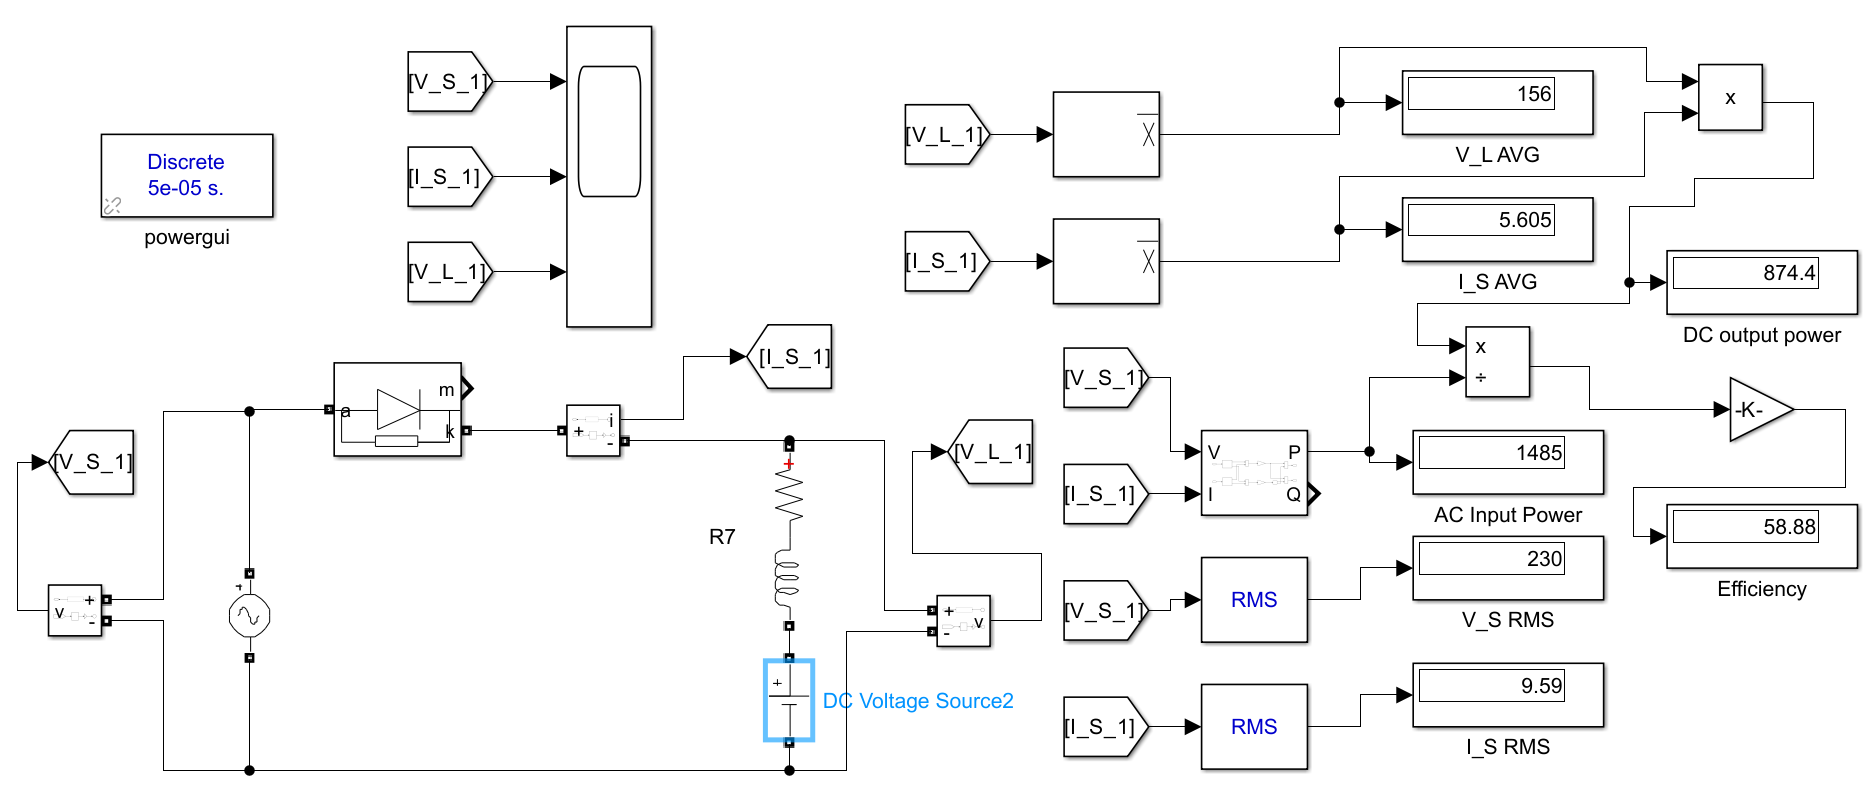
\includegraphics[width=1.0\textwidth]{images/experiment-1/circuit-diagram-experiment-04.png}
    \caption{Circuit for Single Phase Half Wave Uncontrolled Rectifier with RLE load}
    \label{Fig_simulation_circuit_single-phase-half-wave-uncontrolled-rectifier-with-RLE-load}
\end{figure}

\subsection{Components Required}

\begin{table}[h]
    \renewcommand{\arraystretch}{1.3}
    \label{table_components_required_single-phase-half-wave-uncontrolled-rectifier-with-RLE-load}
    \centering
    \begin{tabular}{|c|c|c|c|}
        \hline
        Sr. No & Parameters                     & Ratings            & Quantity \\
        \hline
        \hline
        1      & AC Single Phase Voltage Source & 230V ($ V_{rms} $) & 1        \\
        \hline
        2      & Resistor                       & 10$ \Omega $       & 1        \\
        \hline
        3      & Inductor                       & 10mH               & 1        \\
        \hline
        4      & Diode                          & -                  & 1        \\
        \hline
        5      & DC Source                      & 100V               & 1        \\
        \hline
        6      & Voltmeter                      & -                  & 2        \\
        \hline
        7      & Ammeter                        & -                  & 1        \\
        \hline
    \end{tabular}
    \caption{Components for Single Phase Half Wave Uncontrolled Rectifier with RLE load}
\end{table}




\subsection{Observations}

\begin{table}[h]
    \renewcommand{\arraystretch}{1.3}

    \label{table_observation_single-phase-half-wave-uncontrolled-rectifier-with-RLE-load}
    \centering
    \begin{tabular}{|c|c|c|}
        \hline
        Parameters                              & Theoretical Values & Simulation Values \\
        \hline
        \hline
        AC Input Voltage ($ V_{in,rms} $)       & 230V               & 230V              \\
        \hline
        Output Average Voltage ($ V_{o,avg} $)  & 148V               & 156V            \\
        \hline
        Output Average Current ($ I_{o,avg}  $) & 5.8A               & 5.605A            \\
        \hline
        AC Input Power ($ P_{AC}  $)            & 2389.5 (W)         & 1485 (W)          \\
        \hline
        DC Input Power ($ P_{DC}  $)            & 1071.53 (W)        & 874.4 (W)         \\
        \hline
        Efficiency (\%)                         & 44.84              & 58.88             \\
        \hline
    \end{tabular}
    \caption{Observations for Single Phase Half Wave Uncontrolled Rectifier with RLE load}
\end{table}


Upon observation of the simulation, it has been determined that the output voltage waveform of the single-phase half-wave rectifier mimics that of the RL load. However, it differs in that it always remains positive, and once the output current reaches zero, the diode ceases to conduct, and the output voltage becomes stabilized at 100V.
The efficiency of uncontrolled rectifier with RLE load is 67.88%.

\pagebreak

\subsection{Resultant Waveforms}

% figure that is centered on the page
\begin{figure}[h]
    \centering
    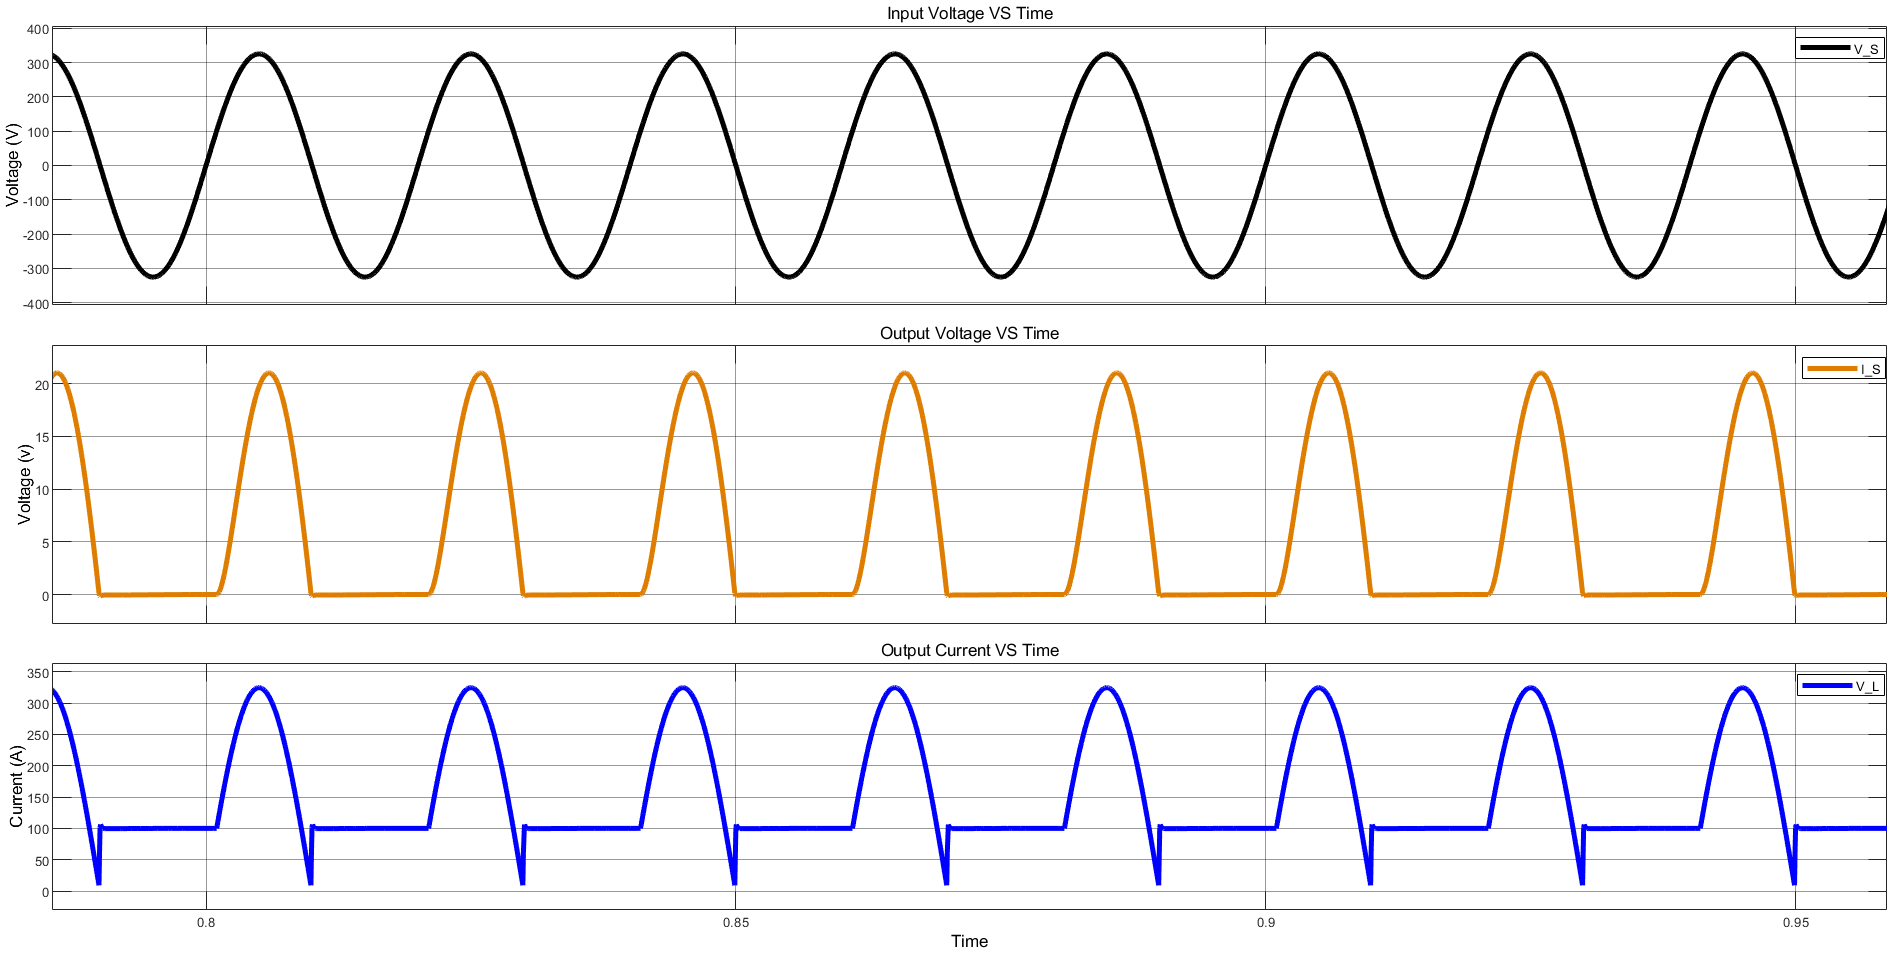
\includegraphics[width=1\textwidth]{images/experiment-1/circuit-scope-experiment-04.png}
    \caption{Scope Waveforms for Single Phase Half Wave Uncontrolled Rectifier with RLE load waveforms}
    \label{Fig_waveform_single-phase-half-wave-uncontrolled-rectifier-with-RLE-load}
\end{figure}

\pagebreak

